\chapter{The Comprehension Test} 

\section{Research questions and hypotheses}\label{sec:05:1}

In line with the overall approach of this research, the comprehension test probes the learner's use of case endings by manipulating word order, based on the assumption that while the meaning of SO targets can be derived based on both a positional and a morphosyntactic principle, on OS targets only the morphosyntactic principle is adequate, as the subject of the utterance no longer occurs in its canonical initial position. Two values of OS word order are considered, i.e. OVS and OSV.

The learners’ performance on OS targets thus makes it possible to quantify the extent to which inflectional morphology plays a role in identifying syntactic functions in comprehension.

\section{Results}\label{sec:05:2}
\subsection{Descriptive statistics}\label{sec:05:2.1}

This section first presents descriptive statistics relative to learner data, then attempts to identify any statistically significant tendencies using a statistical model. The following section will interpret the same data from the viewpoint of the approach described in Section \ref{sec:04:2.4}, with the aim to detail the individual set of skills of each learner.

\figref{fig:05:1} graphically displays learner scores on SVO, OSV and OVS targets at T1.

\begin{figure}
    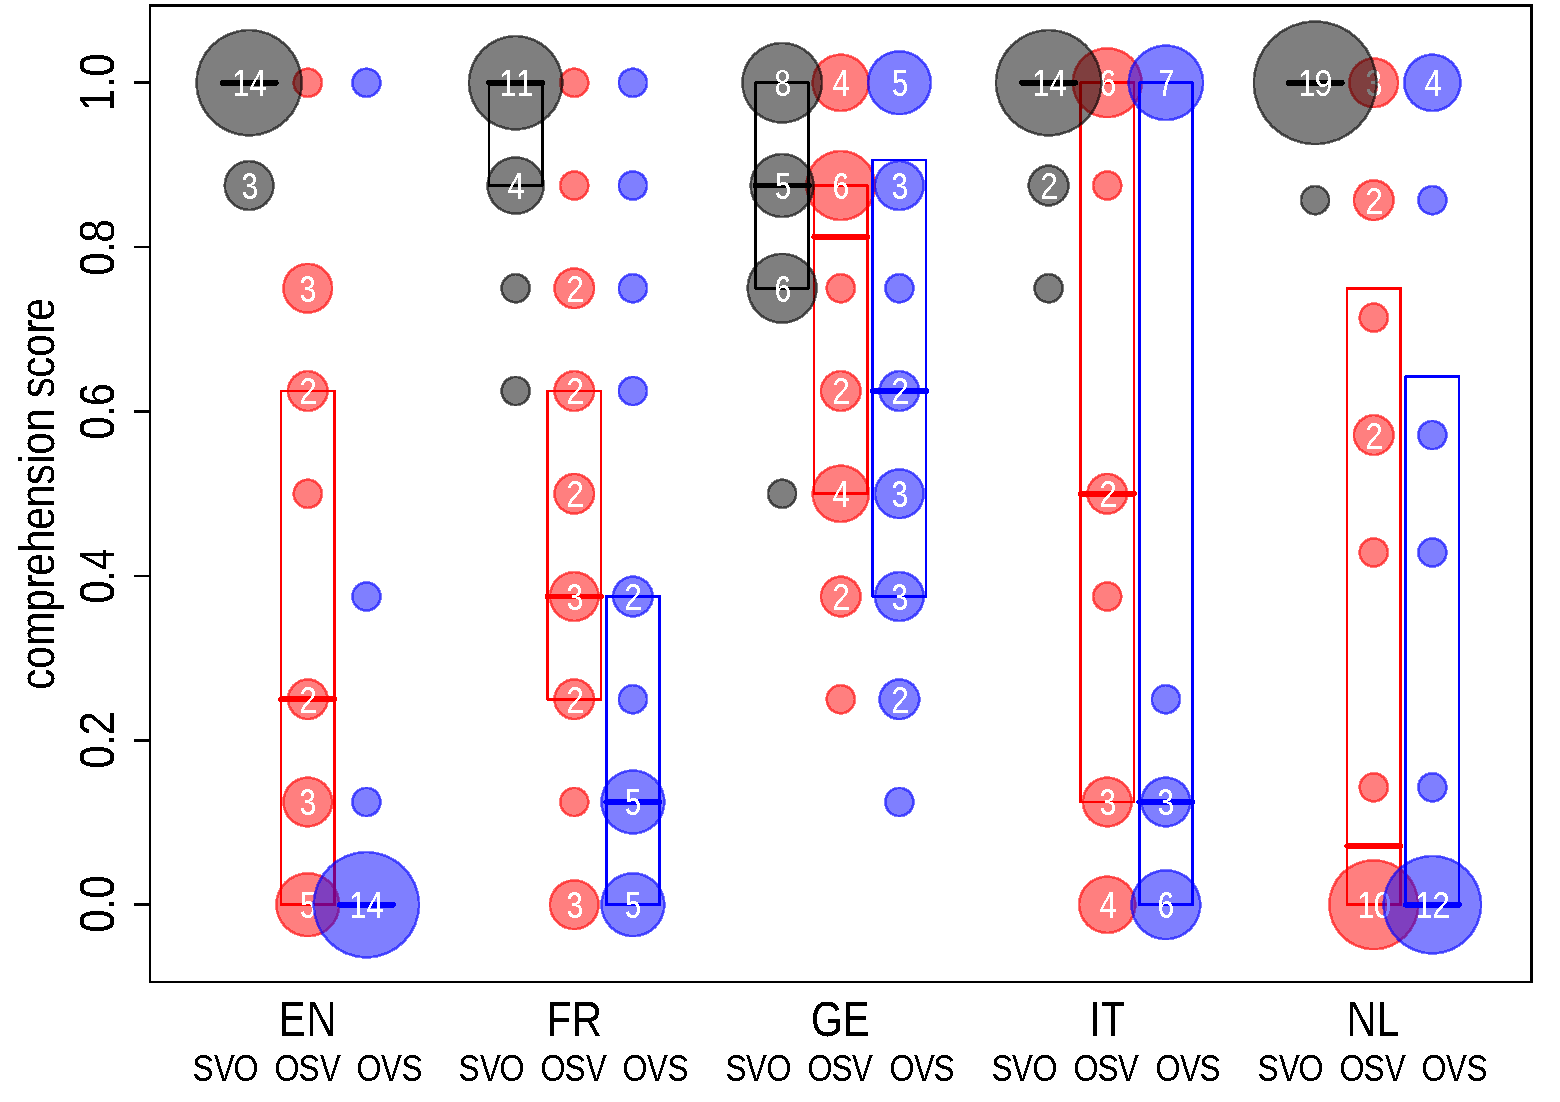
\includegraphics[width=\textwidth]{figures/05-1.pdf}
    \caption{Comprehension test, scores by L1 and word order, T1}
    \label{fig:05:1}
\end{figure}

Descriptive statistics are provided in \tabref{tab:05:1}.

\begin{table}
    \begin{tabularx}{\textwidth}{XXXXXXXX}
    \lsptoprule
    L1 &  & \multicolumn{2}{X}{SVO} & \multicolumn{2}{X}{OSV} & \multicolumn{2}{X}{OVS}\\
    & n. & mean & sd & mean & sd & mean & sd\\
    \cmidrule{2-8}
    EN & 17 & 0.98 & 0.15 & 0.35 & 0.48 & 0.09 & 0.28\\
    FR & 17 & 0.93 & 0.25 & 0.43 & 0.50 & 0.29 & 0.45\\
    GE & 20 & 0.87 & 0.34 & 0.71 & 0.45 & 0.64 & 0.48\\
    IT & 17 & 0.97 & 0.17 & 0.51 & 0.50 & 0.45 & 0.50\\
    NL & 20 & 0.99 & 0.08 & 0.36 & 0.48 & 0.30 & 0.46\\
    mean & {}- & 0.95 & 0.20 & 0.47 & 0.48 & 0.35 & 0.43\\
    \lspbottomrule
    \end{tabularx}
    \caption{Comprehension task, descriptive statistics, T1}
    \label{tab:05:1}
\end{table}

\figref{fig:05:2} graphically displays learner scores on SVO, OSV and OVS targets at T1.

\begin{figure}
    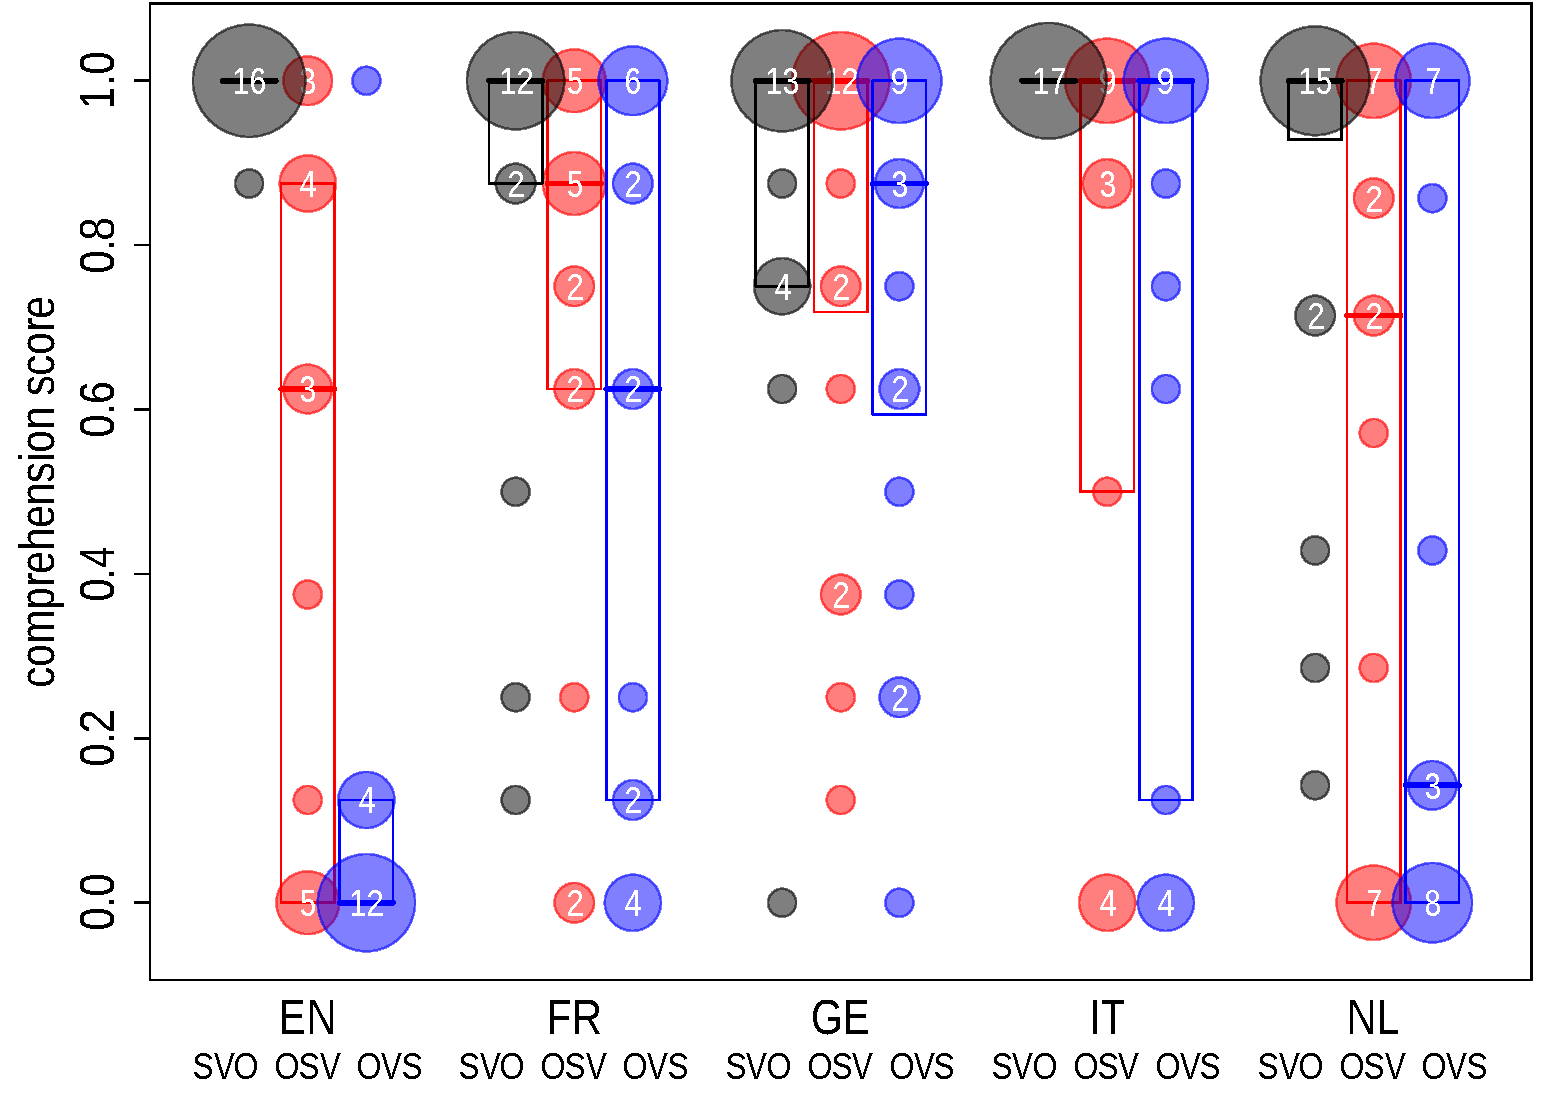
\includegraphics[width=\textwidth]{figures/05-2.pdf}
    \caption{Comprehension test, scores by L1 and word order, T1}
    \label{fig:05:2}
\end{figure}

Descriptive statistics are provided in \tabref{tab:05:2}.

\begin{table}
    \begin{tabularx}{\textwidth}{XXXXXXXX}
    \lsptoprule
    L1 &  & \multicolumn{2}{X}{SVO} & \multicolumn{2}{X}{OSV} & \multicolumn{2}{X}{OVS}\\
    & n. & mean & sd & mean & sd & mean & sd\\
    \cmidrule{2-8}
    EN & 17 & 0.99 & 0.08 & 0.52 & 0.50 & 0.08 & 0.28\\
    FR & 17 & 0.86 & 0.34 & 0.72 & 0.44 & 0.55 & 0.49\\
    GE & 20 & 0.87 & 0.33 & 0.80 & 0.39 & 0.75 & 0.43\\
    IT & 17 & 1.00 & 0.00 & 0.71 & 0.45 & 0.66 & 0.47\\
    NL & 20 & 0.86 & 0.34 & 0.55 & 0.49 & 0.43 & 0.49\\
    mean & {}- & 0.92 & 0.22 & 0.66 & 0.45 & 0.49 & 0.43\\
    \lspbottomrule
    \end{tabularx}
    \caption{Comprehension task, descriptive statistics, T2}
    \label{tab:05:2}
\end{table}

A few preliminary remarks can be made based on these descriptive statistics. First, as expected, SO scores are much higher than their OS equivalents in all cases. Curiously, though, the mean scores below 100\% as well as the rather high standard deviations point to the fact that some learners actually made several errors on SVO targets too, which runs contrary to the initial hypotheses. 

Regularities are also observed in the difference between the two OS constituent orders. Accuracy on OSV targets is higher in all cases, the only exception being the German group at T2. The English group stands out in this respect, too, in that the difference between the two values of word order is particularly extreme, and the standard deviation on OVS targets is much lower than in the other L1 groups. Combined, these two pieces of information indicate that compared to OSV targets, English learners perform much worse on OVS ones than the other L1 groups do, and that all learners in this group do so in a rather uniform manner. 

\subsection{Inferential statistics}\label{sec:05:2.2}

A generalised linear mixed model with binomial error structure and logit link function (Likelihood Type 3-test) was fitted to the data using the R package \textit{lme4} \citep{BatesEtAl2015}: fixed effects comprise the L1 (factor, five levels: EN, FR, GE, IT, NL, reference level=EN), word order (factor, binary, reference level=OS) and time (factor, binary, reference level=1) as linear predictors, as well as their two-way interactions: L1:word order, L1:time, and time:word order. 

The rationale for including the interactions is as follows. The learners' ability to identify the syntactic structure of the target is hypothesised to be influenced by target sentence word order, SO generally having a positive effect, OS having a negative effect. In turn, the impact of word order may be modulated by the learner’s L1. Further exposure is thought to be generally beneficial, but the extent to which results improve between T1 and T2 may be also determined by the learners’ L1 (speakers of certain languages improving more markedly than speakers of other languages) and word order (within the same L1 group, either word order may show greater improvement over time). 

To simulate individual variability, finally, the model includes random intercepts for participants and test items as well as interacting random slopes for word order and time. The model output is presented in \tabref{tab:05:3}.

\begin{table}
    \begin{tabularx}{\textwidth}{XXXX}
    \lsptoprule
    \textbf{~} & \multicolumn{3}{X}{ \textbf{response}}\\
    \textit{Predictors} & \textit{Odds} \textit{Ratios} & \textit{CI} & \textit{p}\\
    \midrule
    (Intercept) & 0.08 & 0.02~–~0.39 & \textbf{0.002}\\
    time [2] & 3.26 & 0.87~–~12.21 & 0.080\\
    L1 [FR] & 4.97 & 0.63~–~38.99 & 0.127\\
    L1 [GE] & 53.17 & 7.05~–~400.88 & \textbf{<0.001}\\
    L1 [IT] & 11.26 & 1.33~–~95.56 & \textbf{0.026}\\
    L1 [NL] & 3.00 & 0.39~–~23.02 & 0.290\\
    WO2 [SO] & 2367.21 & 332.20~–~16868.10 & \textbf{<0.001}\\
    time [2] * L1 [FR] & 2.86 & 0.45~–~18.22 & 0.265\\
    time [2] * L1 [GE] & 1.87 & 0.30~–~11.64 & 0.504\\
    time [2] * L1 [IT] & 4.30 & 0.57~–~32.21 & 0.156\\
    time [2] * L1 [NL] & 1.51 & 0.24~–~9.62 & 0.665\\
    time [2] * WO2 [SO] & 0.36 & 0.18~–~0.75 & \textbf{0.006}\\
    L1 [FR] * WO2 [SO] & 0.02 & 0.00~–~0.18 & \textbf{0.001}\\
    L1 [GE] * WO2 [SO] & 0.00 & 0.00~–~0.01 & \textbf{<0.001}\\
    L1 [IT] * WO2 [SO] & 0.06 & 0.00~–~0.70 & \textbf{0.025}\\
    L1 [NL] * WO2 [SO] & 0.09 & 0.01~–~0.86 & \textbf{0.036}\\
    \multicolumn{4}{X}{\textbf{Random} \textbf{Effects}}\\
    σ\textsuperscript{2} & \multicolumn{3}{X}{3.29}\\
    τ\textsubscript{00}~\textsubscript{participant} & \multicolumn{3}{X}{8.33}\\
    τ\textsubscript{00}~\textsubscript{target\_no} & \multicolumn{3}{X}{0.56}\\
    τ\textsubscript{11}~\textsubscript{participant.time2} & \multicolumn{3}{X}{5.63}\\
    τ\textsubscript{11}~\textsubscript{participant.WO2SO} & \multicolumn{3}{X}{6.98}\\
    ρ\textsubscript{01}~\textsubscript{participant.time2} & \multicolumn{3}{X}{{}-0.11}\\
    ρ\textsubscript{01}~\textsubscript{participant.WO2SO} & \multicolumn{3}{X}{{}-0.93}\\
    ICC & \multicolumn{3}{X}{0.73}\\
    N~\textsubscript{participant} & \multicolumn{3}{X}{91}\\
    N~\textsubscript{target\_no} & \multicolumn{3}{X}{24}\\
    \midrule
    Observations & \multicolumn{3}{X}{4248}\\
    Marginal R\textsuperscript{2}~/ Conditional R\textsuperscript{2} & \multicolumn{3}{X}{0.334 / 0.818}\\
    \lspbottomrule
    \end{tabularx}
    \caption{Output model}
    \label{tab:05:3}
\end{table}

The three hypothesised interactions were probed by comparing this full model to three null models, each lacking the single interaction of interest. Statistical significance was assessed based on likelihood ratio tests (\tabref{tab:05:4}). Multiple comparison was addressed using the Holm correction.

\begin{table}
    \begin{tabularx}{\textwidth}{XXXX}
    \lsptoprule
    predictor & Chisq & Df & Pr(>Chisq)\\
    \midrule
    time : L1 & 2.484 & 4 & >0.05\\
    time : word order & 7.599 & 1 & 0.01\\
    L1 : word order & 35.840 & 4 & <0.01\\
    \lspbottomrule
    \end{tabularx}
    \caption{Comprehension results, single term deletion}
    \label{tab:05:4}
\end{table}

The interaction between time and L1 does not reach statistical significance, but both terms engage in other statistically significant interactions. The latter were explored through pairwise comparisons. In \figref{fig:05:3} and \ref{fig:05:4}, blue bars depict confidence intervals: for any pairwise comparison, two terms differ significantly if the red arrows do not overlap.

\figref{fig:05:3} depicts the interaction between time and word order. No statistically significant difference between T1 and T2 can be observed for SO targets, which indicates no significant improvement in time. The reverse is true for OS targets, in which a statistically significant improvement can be observed between T1 and T2 for all L1 groups except the L1 English group, whose performance does improve in time, but not to a significant extent.

\begin{figure}
    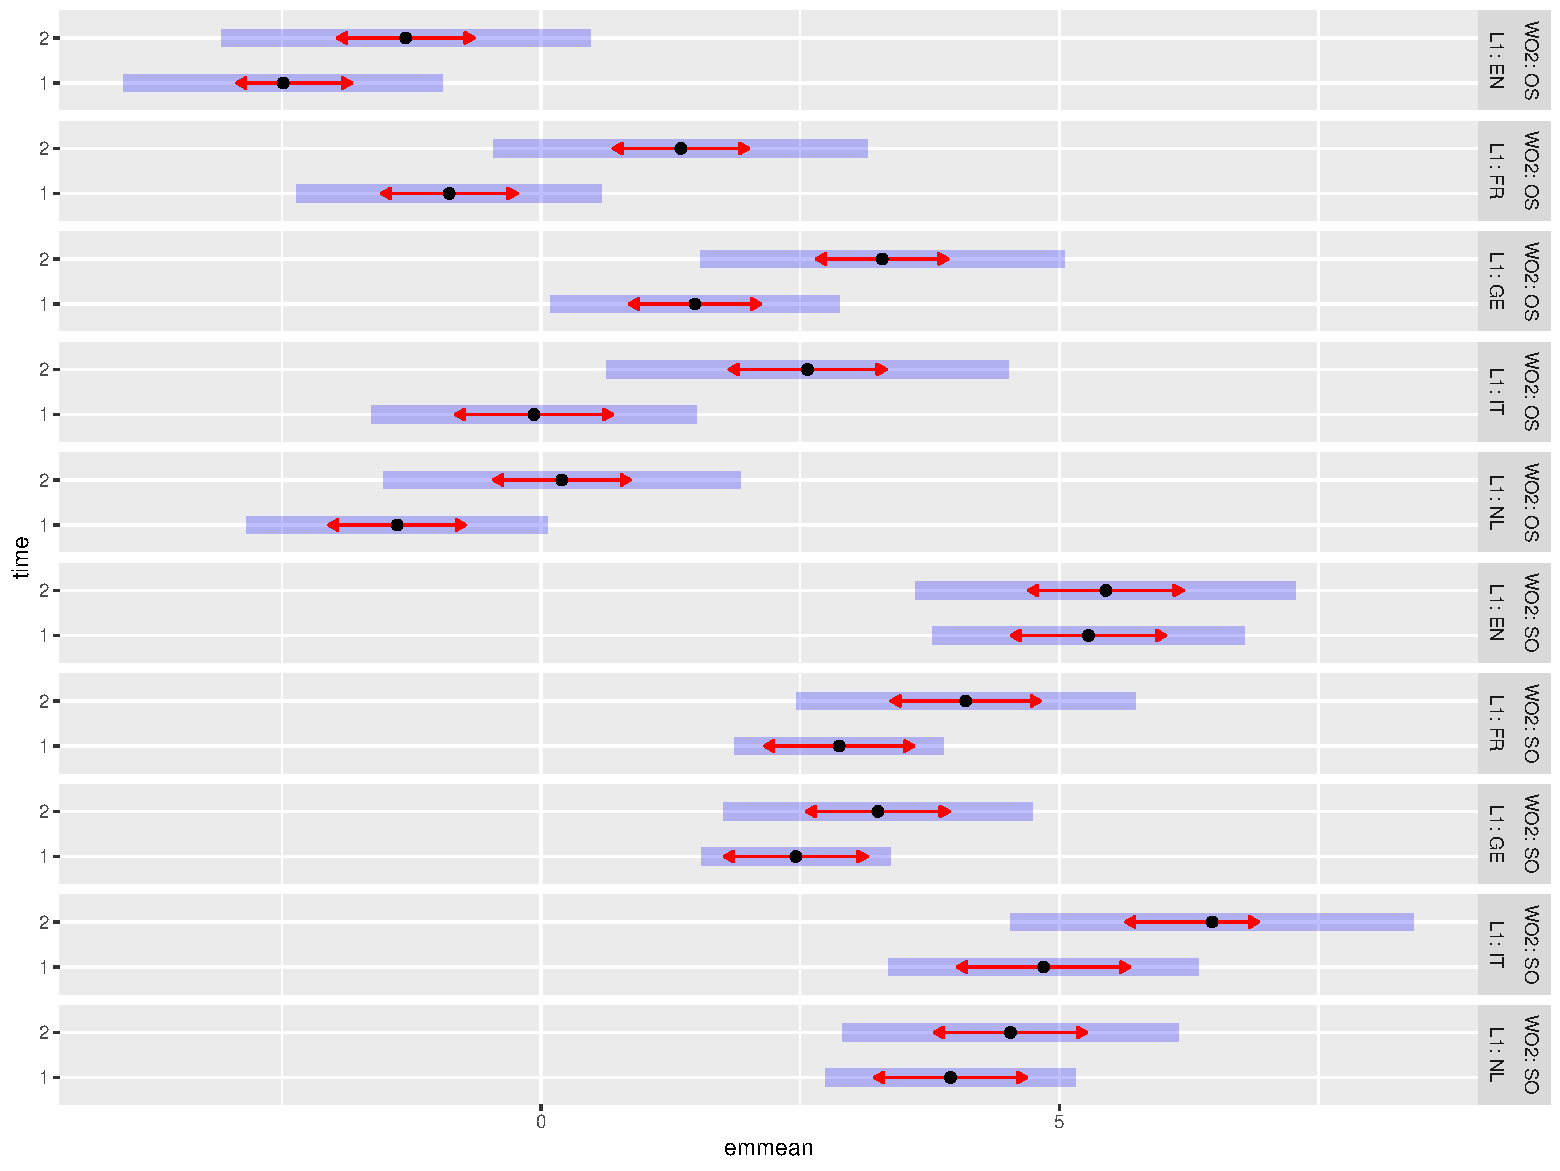
\includegraphics[width=\textwidth]{figures/05-3.pdf}
    \caption{Pairwise comparisons, effect of time across L1 and word order}
    \label{fig:05:3}
\end{figure}

\figref{fig:05:4} depicts the interaction between L1 and word order. Notable facts are reported in \tabref{tab:05:5}. The symbols “>” and “<” indicate significantly better and significantly worse performance, respectively. Only significant contrasts are reported.

\begin{table}
    \begin{tabularx}{\textwidth}{ll}
    \lsptoprule
    condition & significant contrasts\\
    \midrule
    T1, OS & GE > NL (p = 0.03), EN (p < 0.01)\\
    T1, SO & GE < IT (p = 0.01), EN (p < 0.01);
    
    FR < EN (p = 0.02)\\
    T2, OS & EN < GE (p < 0.01), IT (p = 0.02)\\
    T2, SO & GE < IT (p = 0.03)\\
    \lspbottomrule
    \end{tabularx}
    \caption{Pairwise comparisons, L1: word order (WO) interaction, significant contrasts}
    \label{tab:05:5}
\end{table}

\begin{figure}
    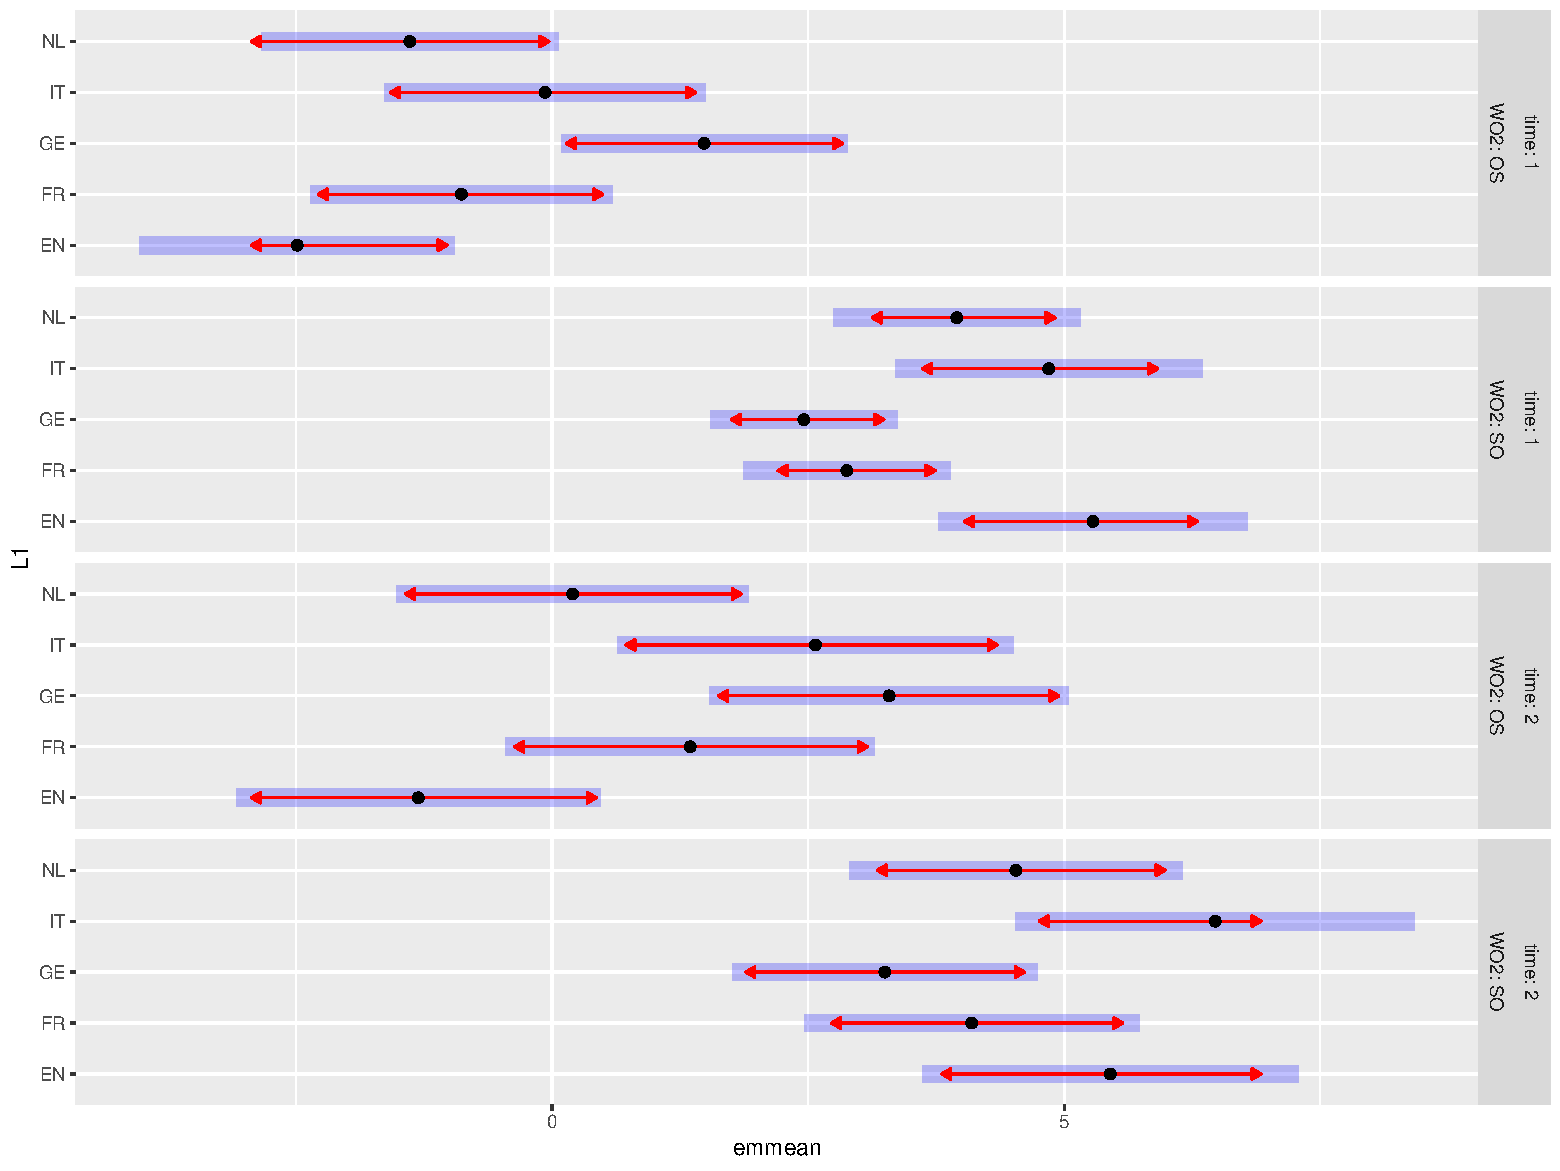
\includegraphics[width=\textwidth]{figures/05-4.pdf}
    \caption{Pairwise comparisons, effect of L1 across time and word order}
    \label{fig:05:4}
\end{figure}

\subsection{Individual processing strategies}\label{sec:05:2.3}

Based on the approach discussed in Section \ref{sec:04:2.4}, this section attempts to compute the likelihood that learners might have performed the Comprehension test with above chance level accuracy, that is, that they responded correctly in such a consistent and systematic way that the existence of a morpho-syntactic principle of utterance organisation may be hypothesised. 

\figref{fig:05:5} shows the number of participants who can be said to have applied a target-like morphosyntactic principle in their responses to the comprehension task at T1 (target-like behaviour was defined as systematic, above-chance performance). The digits indicate the actual number of participants for each category.

\begin{figure}
    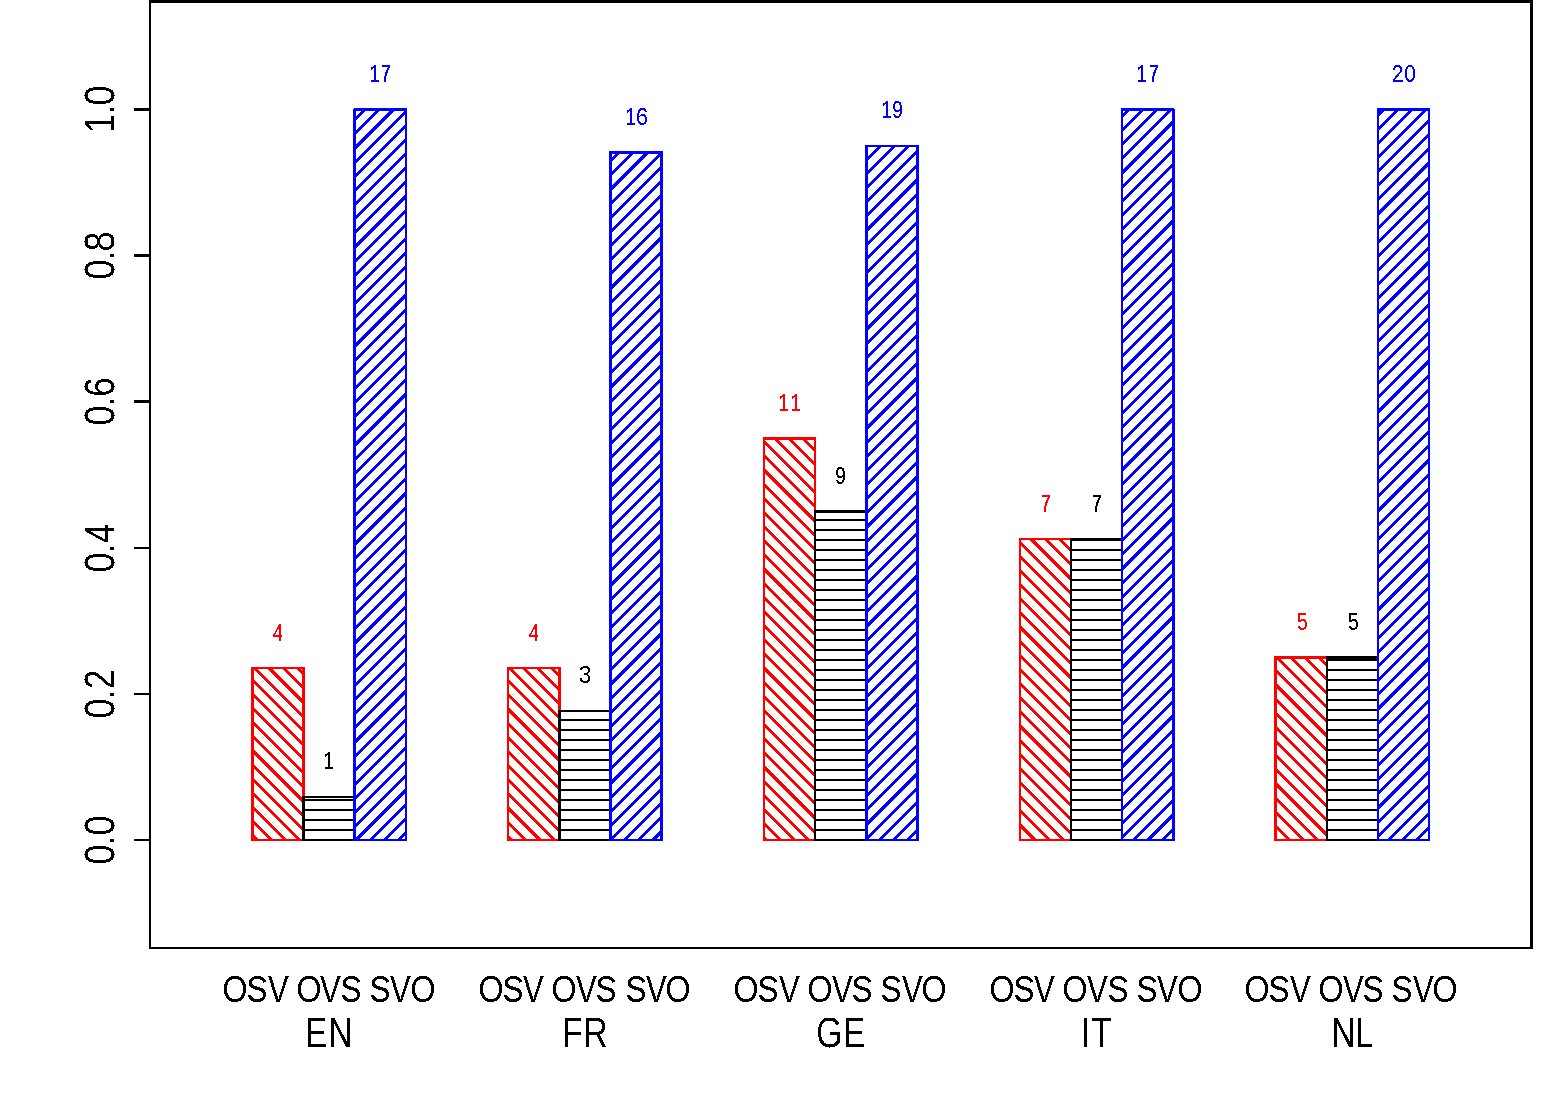
\includegraphics[width=\textwidth]{figures/05-5.pdf}
    \caption{Comprehension task, learner above chance}
    \label{fig:05:5}
\end{figure}

The first noteworthy observation concerns the obvious difference between the processing of SO targets, on the one hand, and of OS ones, on the other hand. It is curious that two learners (one German, one French) did not achieve above chance accuracy on this type of targets. 

Nevertheless, quite a few participants seemed able to correctly process OS targets: this regards 31 learners on OSV and 25 on OVS targets. All L1s are represented, although values for the Italian and German groups are higher than others. 

The two values of OS (OSV and OVS) appear to be very similar. If a difference exists, it is very slight and in favour of OSV. 

\figref{fig:05:6} presents the data at T2.

\begin{figure}
    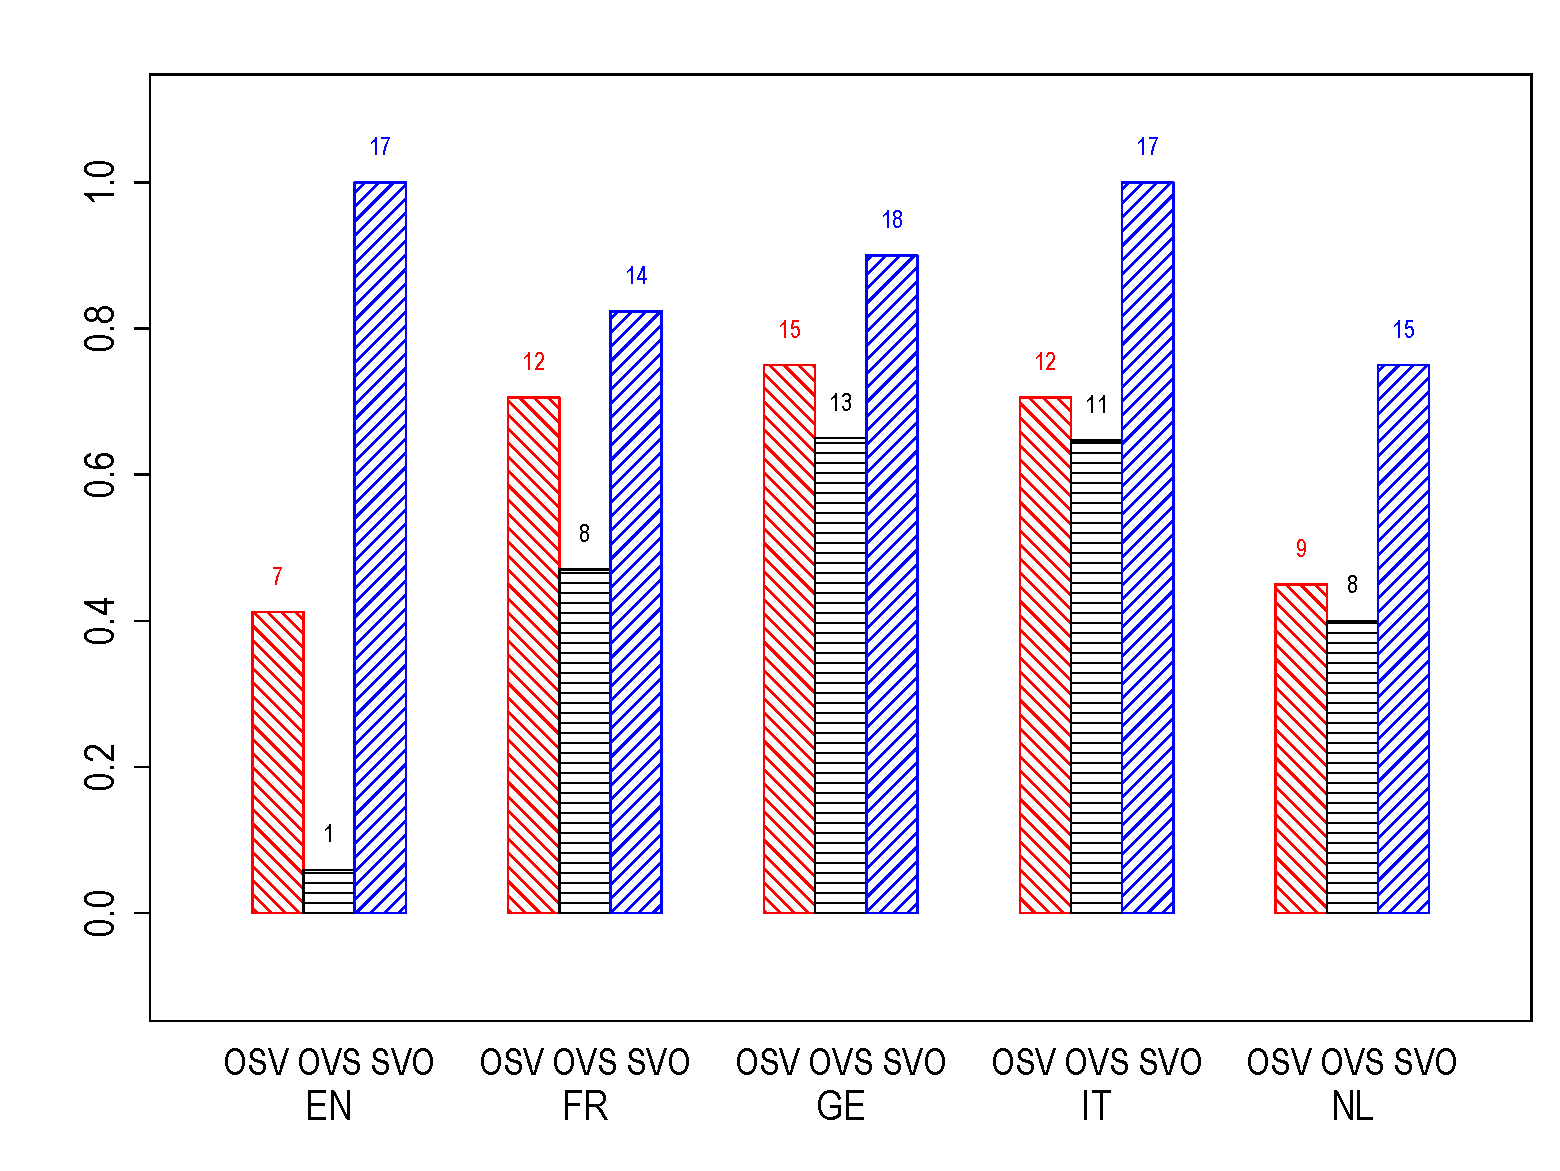
\includegraphics[width=\textwidth]{figures/05-6.pdf}
    \caption{Learners significantly above chance by L1, comprehension task}
    \label{fig:05:6}
\end{figure}

Two main tendencies can be observed. The first concerns the marked increase in the number of learners with above chance level accuracy in the processing of OS targets, which grows in all L1 groups. With the only exception of the L1 English group, the improvement concerns both values of OS, although the advantage of OSV over OVS remains. Although less evidently than at T1, the L1 Italian and L1 German groups still achieve better performance than the other groups.

Second, the number of learners failing to reach above chance accuracy on SO also increases.

\subsection{A comprehensive picture}\label{sec:05:2.4}

Data can also be displayed so that the scores of each individual learner may be synoptically seen as a function of L1, word order, and time. The objective is to perform a simple cluster analysis to verify whether learners can be grouped based on these factors. 

In \figref{fig:05:3}, T1 and T2 scores are presented on the horizontal (black) and on the vertical (red) axis, respectively. On both axes, scores are defined by the combination of learner performance on the three target word orders: SVO, OVS and OSV. A score of 1 indicates that the learner performs above chance on the corresponding target structure, whereas 0 indicates response at chance level. 

Learners are thus identified by a combination of scores at T1 (horizontal axis, black) and T2 (vertical axis, red), that is, by their position in one of the 64 squares in which the graph area is divided. Each data point represents an individual learner, whose L1 is also specified.

\begin{figure}
    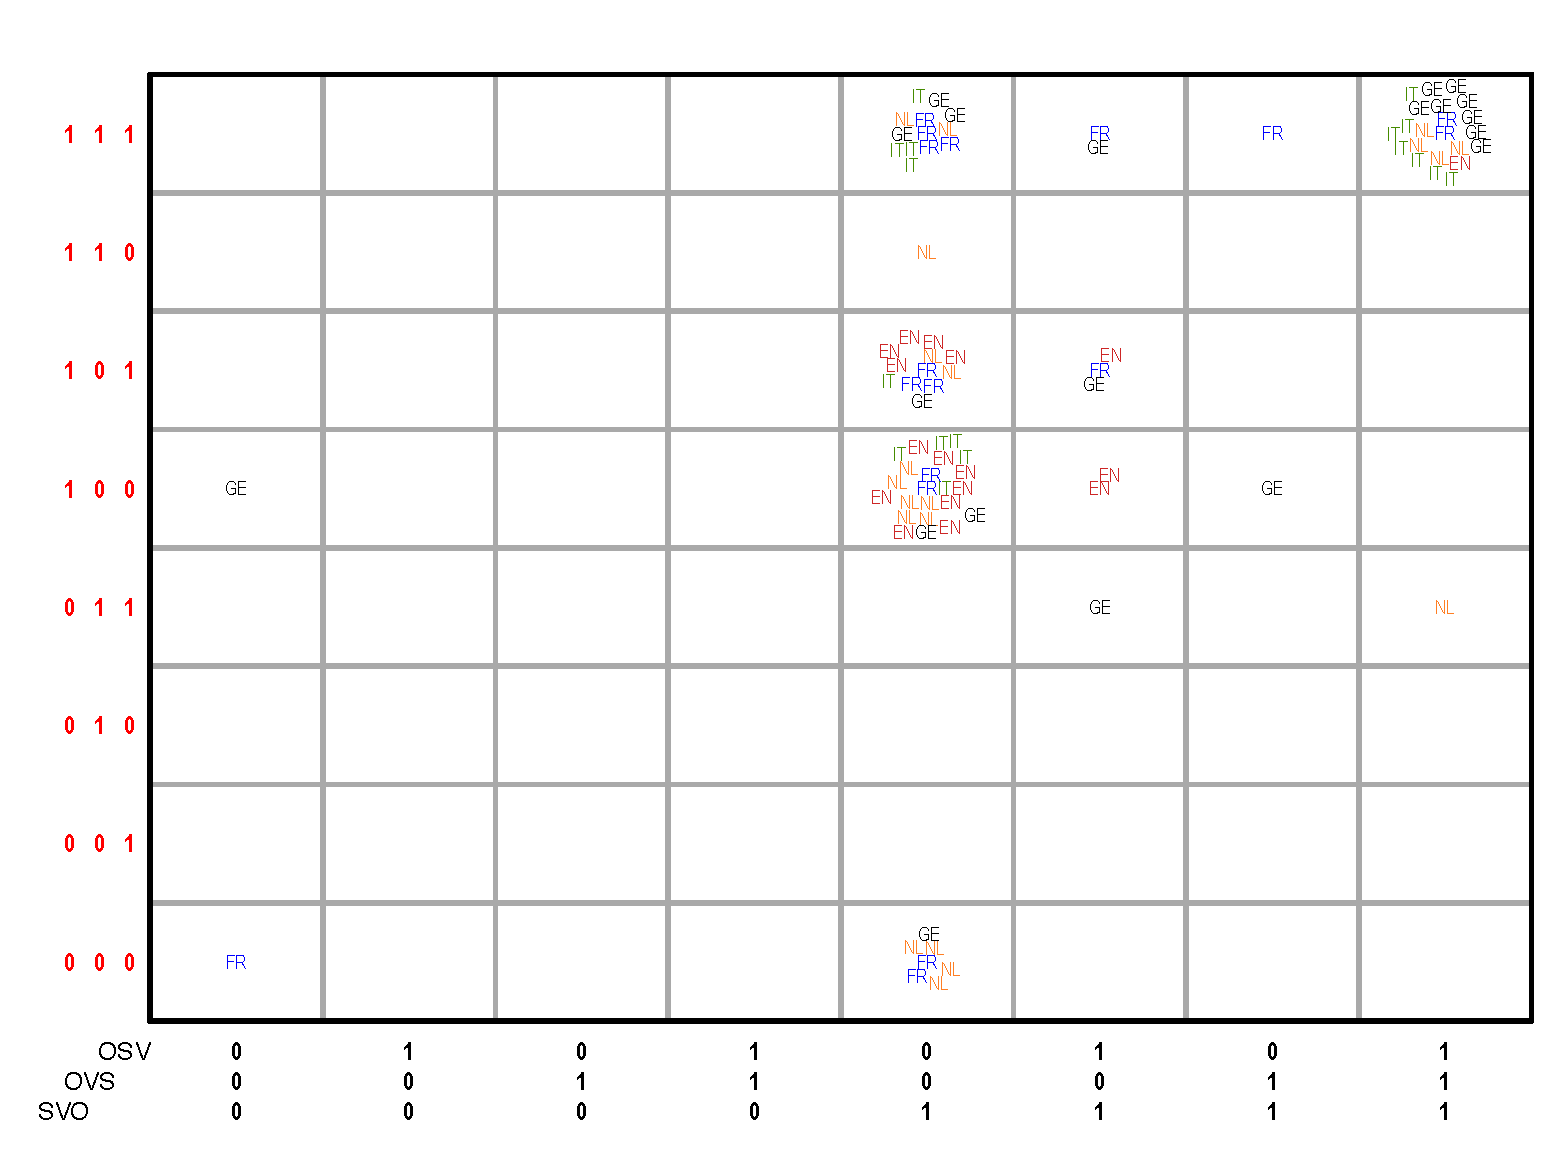
\includegraphics[width=\textwidth]{figures/05-7.pdf}
    \caption{Comprehension task, individual processing strategies}
    \label{fig:05:7}
\end{figure}

Out of the 64 theoretically possible scenarios, only a few are realised in practice, and fewer still include the bulk of the subjects. As each square corresponds to a varying degree of success in the test, i.e. on various types of targets, one could interpret this information as a hint to the existence of a hierarchy in the development of morphosyntactic competence in comprehension, identifiable both synchronically and diachronically. For a synchronic analysis, one needs to consider the column sum, for T1, or the row sum, for T2, in order to compute the number of participants performing in a specific manner at either test time. 

It is evident that at T1 most learners (56) show the following score: SVO 1, OVS 0, OSV 0, which corresponds to a clear positional strategy. 23 learners, in contrast, already exhibit a well-developed morphosyntactic strategy (SVO 1, OVS 1, OSV 1). In between these two groups, 8 learners correctly process SVO and OSV targets, but not OVS, and only 2 do the opposite, which suggests that OSV structures should be more accessible compared to their OVS equivalents. 

At T2, the number of learners applying a pure positional principle (fourth line in the graph) is reduced to 26, whereas those always using a morphosyntactic strategy (first line) now number 36. 15 participants, finally, perform better on OSV than OVS targets. The picture at T2, therefore, confirms the situation at T1, with a tendency for results to become more target-like.

One can also study the evolution of learners' processing strategies over time. It seems most relevant to describe the potential evolution of the 56 participants who at T1 were found to adopt a pure positional strategy (SVO 1, OVS 0, OSV 0). 23 of them did not change their processing strategy, consistently applying the same strategy at T2 as well. In contrast, 13 participants moved all the way towards a morphosyntactic strategy, so that at T2 they proved able to consistently derive meaning from both SO and OS targets. 12 learnt to process OSV structures, but still not OVS; only 1 learner exhibits the reverse evolution. This information fits in with the synchronic data, which showed that at both T1 and T2 OSV targets are correctly processed by a greater number of learners than their OVS equivalents. Diachronically, it appears that case-marking in the two OS word orders can develop either at same time, or separately, in which case OSV develops first. 

Finally, 7 subjects (last line, fifth column) move to a stage in which no word order is processed above chance. Beside the fact that additional exposure to the input is apparently detrimental to these learners, this last scenario is particularly surprising in light of the fact that the meaning of SO targets can be correctly identified based on a positional principle.

\subsection{Differential processing of OS word orders}\label{sec:05:2.5}

The analysis so far has revealed obvious gaps in scores between SO targets, on the one hand, and OS targets, on the other hand. These differences are not problematic in that they can easily be explained by the processing principle required to extract meaning from them: positional or morphosyntactic in the former case, necessarily morphosyntactic in the latter. When it comes to OS targets, however, there should be no differences in processing accuracy, as both OSV and OVS targets share the same relative order of subject and object. Nevertheless, it does seem that OVS targets prove consistently harder to process that OSV ones. Evidence for such claim comes from various sources: alongside marked differences in mean scores, the processing of OVS targets was often found not to reach above chance performance; further, scenarios in which, at a given time, OVS structures are processed more accurately than OSV are rare; diachronically, OSV almost always develops before OVS. This section first describes the phenomenon in detail and then reports on a statistical test to verify whether the observed differences are statistically significant and require a specific explanation.

\figref{fig:05:4} presents an overall picture of each learner's processing strategy of OS targets at both T1 and T2. The processing scores of OSV targets are represented on the horizontal axis, with learners behaving at chance level on the left (scenarios 2 and 4), and learners above chance on the right (scenarios 1 and 3). Conversely, the processing scores of OVS targets are represented on the vertical axis, with learners behaving at chance level at the bottom (scenarios 2 and 3) and learners above chance at the top (scenarios 2 and 4). Taken together, the two scores provide an overall picture of learners' behaviour on both OVS and OSV targets at the same time. The main area is divided into four main squares, each representing a processing scenario at T1 according to the conventions summarised in \tabref{tab:05:6}.

\begin{table}
    \begin{tabularx}{\textwidth}{XXXX}
    \lsptoprule
    \multicolumn{2}{X}{} & \multicolumn{2}{X}{OSV}\\
    &  & p ${\leq}$ 0.05 & p > 0.05\\
    \multicolumn{1}{X}{OVS} & p ${\leq}$ 0.05 & 1 & 4\\
    & p > 0.05 & 3 & 2\\
    \lspbottomrule
    \end{tabularx}
    \caption{Scenarios, rationale}
    \label{tab:05:6}
\end{table}

Scenario 1 indicates that the learner processes both OSV (horizontal axis, black) and OVS (vertical axis, red) targets based on a morphosyntactic principle, whereby the first NP is always interpreted as the subject. Scenario 2 is the reverse, that is, both types of target are processed positionally, which leads to an incorrect interpretation of the sentence. In scenario 3, OSV targets are processed in a target-like manner, whereas OVS targets are not; the opposite happens in scenario 4. The last two scenarios are particularly relevant for the present research question, as they suggest a discrepancy in the processing of the two types of OS target.

The main squares are further divided into four smaller squares each, which represent the same processing scenarios, in the same order, but relative to T2. In this manner, an indication of the evolution in time of learner processing strategies is included in the graph. Overall scenarios are identified by the two digits corresponding to learner performance at T1 and T2, in that order.

\begin{figure}
    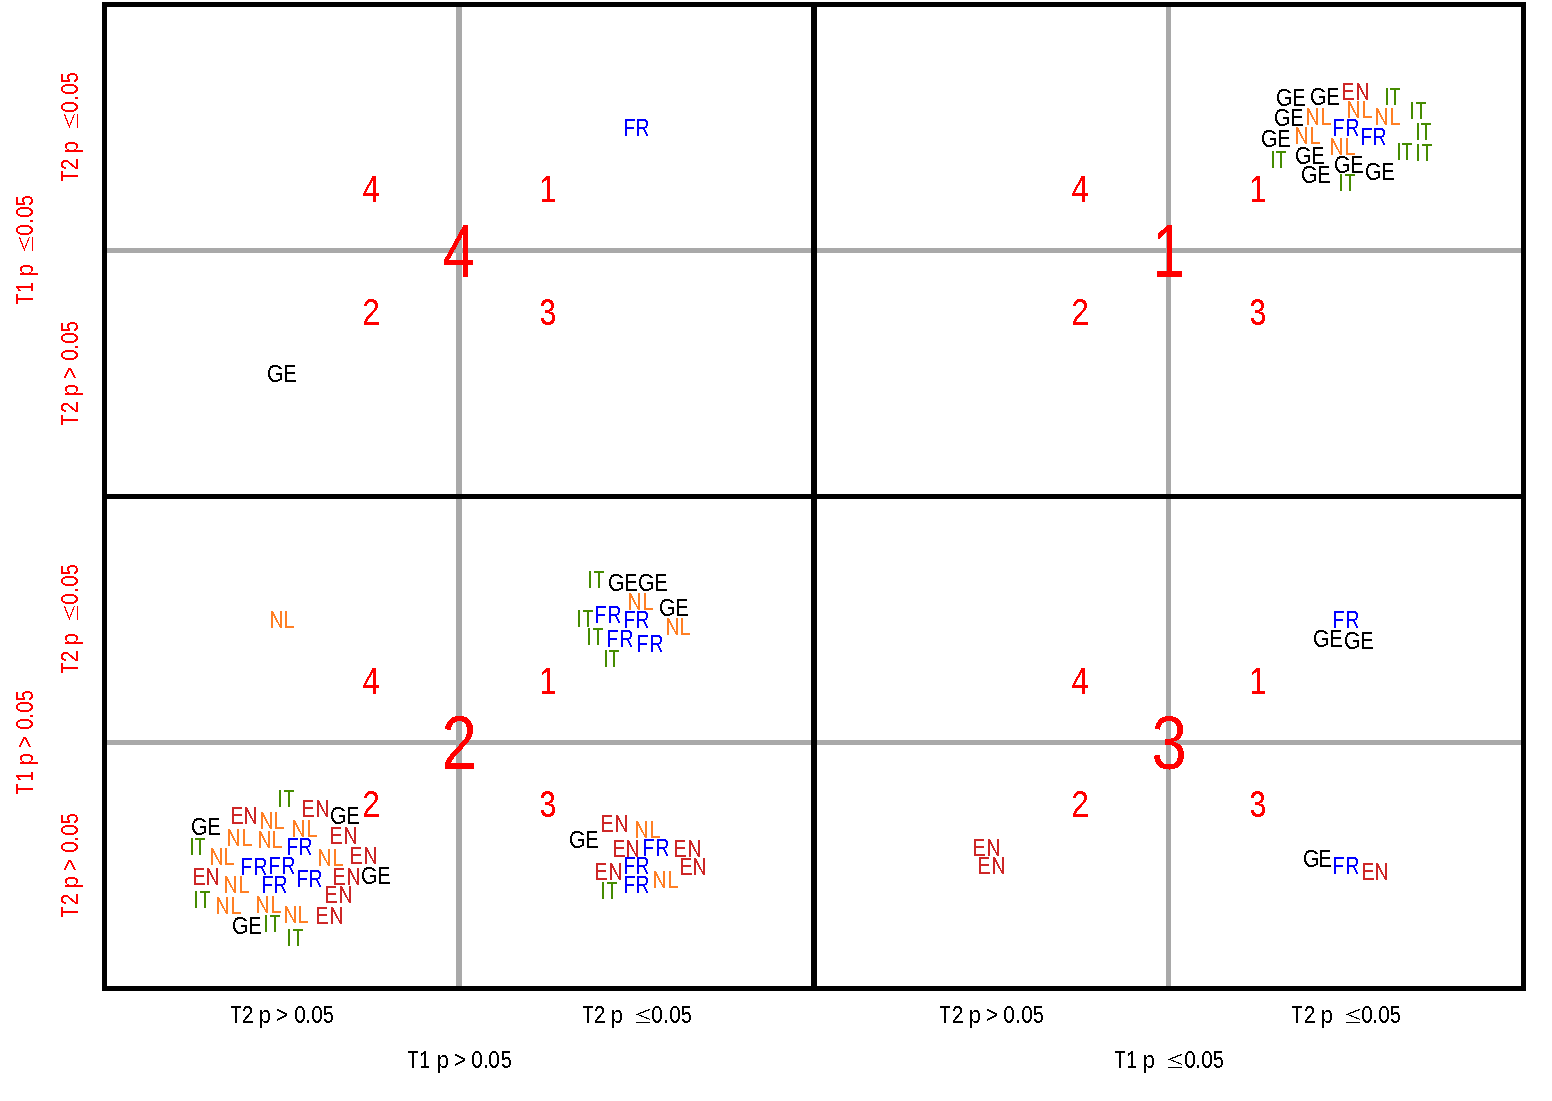
\includegraphics[width=\textwidth]{figures/05-8.pdf}
    \caption{Comprehension task, individual processing strategies, OSV-OVS targets}
    \label{fig:05:8}
\end{figure}

The two main clusters which can be identified concentrate in scenarios 2;2 and 1;1, both representing an extreme picture. In scenario 2;2, learners consistently process both types of OS targets based on a positional principle. Their situation is stable between T1 and T2. 

Conversely, learners in scenario 1;1 apply a target-like morphosyntactic strategy at both test times. 

Two further major clusters originate from scenario 2 at T1, which indicates a positional principle on both types of targets at T1. However, these learners evolve differently with time: those in scenario 2;1 move on to scenario 1 at T2, which means that over time they learnt to generalise a morphosyntactic strategy to all OS targets. Those in scenario 2;3 managed to do so only on OSV targets, and not on OVS ones. The reverse situation, with learners processing correctly OVS targets, but not OSV ones, is only instantiated by a single learner. This suggests that in diachrony, OSV targets tend to be acquired first.

Synchronically, more learners appear in scenario 3 than in scenario 4 at both T1 and T2, as shown in \tabref{tab:05:7} and \ref{tab:05:8} respectively.

\begin{table}
    \begin{tabularx}{\textwidth}{XXXX}
    \lsptoprule
    \multicolumn{2}{X}{} & \multicolumn{2}{X}{OSV}\\
    &  & p ${\leq}$ 0.05 & p > 0.05\\
    \multicolumn{1}{X}{OVS} & p ${\leq}$ 0.05 & 23 & 2\\
    & p > 0.05 & 8 & 58\\
    \lspbottomrule
    \end{tabularx}
    \caption{Comprehension test, OS targets, learner distribution across scenarios, T1}
    \label{tab:05:7}
\end{table}

\begin{table}
    \begin{tabularx}{\textwidth}{XXXX}
    \lsptoprule
    \multicolumn{2}{X}{} & \multicolumn{2}{X}{OSV}\\
    &  & p ${\leq}$ 0.05 & p > 0.05\\
    \multicolumn{1}{X}{OVS} & p ${\leq}$ 0.05 & 40 & 1\\
    & p > 0.05 & 15 & 35\\
    \lspbottomrule
    \end{tabularx}
    \caption{Comprehension test, OS targets, learner distribution across scenarios, T2}
    \label{tab:05:8}
\end{table}

It thus appears that OSV targets are indeed easier to process that OVS; in the following lines a few reasons for this will be explored. In SVO targets \REF{ex:05:1}, agent and patient appear in utterance-initial and utterance-final position respectively, whereas the verb is in utterance-medial position. As SVO is the dominant order in both the target language and the learners' L1s, this structure may be considered to be the prototype of transitive utterances. 

\ea%1
    \label{ex:05:1}
    \gll    {siostr-a}   {woła}   {brat-a}\\
            sister-\textsc{nom}   calls  brother-\textsc{acc}\\
    \glt    `(The) sister calls (her) brother.'
    \z

OVS targets also present the two nouns in utterance-initial and utterance-final position and the verb in utterance-medial position: this time, however, the patient comes first. This structure is therefore identical to SVO as far as the relative order of phrases is concerned. The only way to correctly process this type of targets, or to distinguish them from their SVO equivalents, is to process inflectional morphology.  

\ea%2
    \label{ex:05:2}
    \gll    {brat-a}     {woła}  {siostr-a}\\
            brother-\textsc{acc}  calls  sister-\textsc{nom}\\
    \glt    `(The) sister calls (her) brother.'
    \z

Morphosyntactic processing requires learners to be aware of the gender and inflectional class of target nouns: as \REF{ex:05:2} makes it clear, both nouns may be marked by the same ending, whose meaning (\textsc{nom.sg.f} vs. \textsc{acc.sg.m}) depends on the paradigm to which the noun belongs. Combined with the modest prominence of case endings and the pressure exerted by the test, this may confuse learners, leading them to mistake these targets for instances of SVO utterances. In other words, it may be the case that whenever learners encounter a sentence with the structure NP - V - NP, they interpret it as SVO. It may not be a chance that this tendency is particularly strong with English and French learners, that is, speakers of languages whose word order is particularly rigid, which in turn leads to a very stringent association between the linear order of phrases and meaning.

The picture changes with OSV targets \REF{ex:05:3}, in which the structure of the utterance is quite different: the two noun phrases come first, followed by the verb. This order hardly ever appears in the input, and is therefore unfamiliar to the learners. This seems to be enough for them to notice the difference from the prototype, rather marked in fact, and pay attention to inflectional morphology, or perhaps interpret the utterance as OS simply because it appears so different from the prototypical SVO structure. 

\ea%3
    \label{ex:05:3}
    \gll    {brat-a}     {siostr-a}   {woła}\\
            brother-\textsc{acc}  sister-\textsc{nom}  calls\\
    \glt    `(The) sister calls (her) brother.'
    \z

\subsubsection{Differential processing of OS word orders: Inferential statistics}\label{sec:05:2.5.1}

To test the effect of OS word order statistically, the generalised linear mixed model described in Section \ref{sec:05:2.1} was compared to an identical model, in which however the predictor WO2 (word order with two values, i.e. SO and OS) was substituted with the predictor WO3 (word order with three values, i.e. SVO, OVS and OSV). The model output is presented in \tabref{tab:05:9}.

\begin{table}
    \begin{tabularx}{\textwidth}{lrrr}
    \lsptoprule
    \textbf{~} & \multicolumn{3}{X}{ \textbf{response}}\\
    \textit{Predictors} & \textit{Odds} \textit{Ratios} & \textit{CI} & \textit{p}\\
    \midrule
    (Intercept) & 0.28 & 0.07~–~1.09 & 0.067\\
    time [2] & 4.15 & 0.99~–~17.38 & 0.051\\
    L1 [FR] & 2.33 & 0.38~–~14.30 & 0.360\\
    L1 [GE] & 17.70 & 2.96~–~105.90 & \textbf{0.002}\\
    L1 [IT] & 4.08 & 0.61~–~27.20 & 0.146\\
    L1 [NL] & 1.43 & 0.24~–~8.67 & 0.696\\
    WO3 [OVS] & 0.01 & 0.00~–~0.04 & \textbf{<0.001}\\
    WO3 [SVO] & 681.07 & 111.54~–~4158.79 & \textbf{<0.001}\\
    time [2] * L1 [FR] & 2.52 & 0.34~–~18.69 & 0.367\\
    time [2] * L1 [GE] & 1.31 & 0.18~–~9.44 & 0.787\\
    time [2] * L1 [IT] & 3.28 & 0.38~–~28.23 & 0.280\\
    time [2] * L1 [NL] & 1.18 & 0.16~–~8.65 & 0.872\\
    time [2] * WO3 [OVS] & 1.37 & 0.73~–~2.58 & 0.324\\
    time [2] * WO3 [SVO] & 0.41 & 0.19~–~0.91 & \textbf{0.028}\\
    L1 [FR] * WO3 [OVS] & 31.41 & 4.97~–~198.62 & \textbf{<0.001}\\
    L1 [GE] * WO3 [OVS] & 117.22 & 17.14~–~801.53 & \textbf{<0.001}\\
    L1 [IT] * WO3 [OVS] & 94.50 & 11.59~–~770.64 & \textbf{<0.001}\\
    L1 [NL] * WO3 [OVS] & 37.62 & 5.60~–~252.89 & \textbf{<0.001}\\
    L1 [FR] * WO3 [SVO] & 0.04 & 0.00~–~0.31 & \textbf{0.002}\\
    L1 [GE] * WO3 [SVO] & 0.00 & 0.00~–~0.03 & \textbf{<0.001}\\
    L1 [IT] * WO3 [SVO] & 0.16 & 0.02~–~1.66 & 0.124\\
    L1 [NL] * WO3 [SVO] & 0.19 & 0.02~–~1.61 & 0.129\\
    \multicolumn{4}{X}{\textbf{Random} \textbf{Effects}}\\
    σ\textsuperscript{2} & \multicolumn{3}{X}{3.29}\\
    τ\textsubscript{00}~\textsubscript{participant} & \multicolumn{3}{X}{6.15}\\
    τ\textsubscript{00}~\textsubscript{target\_no} & \multicolumn{3}{X}{0.24}\\
    τ\textsubscript{11}~\textsubscript{participant.time2} & \multicolumn{3}{X}{6.63}\\
    τ\textsubscript{11}~\textsubscript{participant.WO3OVS} & \multicolumn{3}{X}{3.83}\\
    τ\textsubscript{11}~\textsubscript{participant.WO3SVO} & \multicolumn{3}{X}{5.19}\\
    ρ\textsubscript{01}~\textsubscript{participant.time2} & \multicolumn{3}{X}{{}-0.14}\\
    ρ\textsubscript{01}~\textsubscript{participant.WO3OVS} & \multicolumn{3}{X}{0.70}\\
    ρ\textsubscript{01}~\textsubscript{participant.WO3SVO} & \multicolumn{3}{X}{{}-0.91}\\
    ICC & \multicolumn{3}{X}{0.76}\\
    N~\textsubscript{participant} & \multicolumn{3}{X}{91}\\
    N~\textsubscript{target\_no} & \multicolumn{3}{X}{24}\\
    Observations & \multicolumn{3}{X}{4248}\\
    Marginal R\textsuperscript{2}~/ Conditional R\textsuperscript{2} & \multicolumn{3}{X}{0.375 / 0.852}\\
    \lspbottomrule
    \end{tabularx}
    \caption{Model output}
    \label{tab:05:9}
\end{table}

A likelihood-ratio test reveals a statistically significant difference between the two models (Chisq = 131.41, Df = 10, p < 0.01), which suggests that accounting for the differential processing of OS word order configuration is beneficial to the interpretation of the data. However, pairwise comparisons (\figref{fig:05:9}) reveal that the difference in score between the processing of OVS and OSV is significant only for L1 English learners (p < 0.01 at both test times).

\begin{figure}
    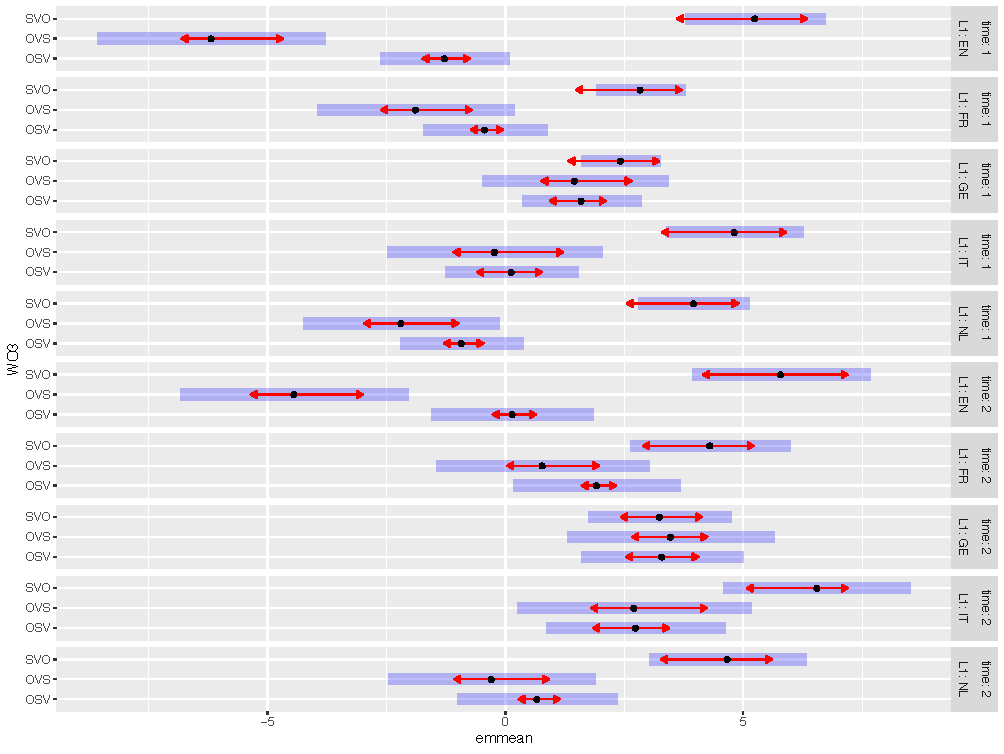
\includegraphics[width=\textwidth]{figures/05-9.pdf}
    \caption{Pairwise comparisons, WO3 across L1 and time}
    \label{fig:05:9}
\end{figure}

\section{Summary}\label{sec:05:3}

This chapter described the results of the Comprehension test, in which learners were asked to listen to a short transitive utterance and to identify its syntactic structure by selecting the appropriate picture. The main findings can be summarised as follows. First, as hypothesised, SO structures are more easily interpreted than their OS equivalent. Second, the learners' familiarity with OS targets increases with time, so that, by T2, a fair half of the subjects can consistently process all target structures. Finally, all L1 groups behave in a comparatively similar manner with the only exception of the English learners, who appear to be much more biased towards a agent-first interpretation of any target structure.
